\documentclass{article}
\usepackage{graphicx, tikz-cd} % Required for inserting images
\usepackage{amsmath, amssymb, amsthm, amsfonts, siunitx, physics}
\AtBeginDocument{\RenewCommandCopy\qty\SI}
\usepackage[version=4]{mhchem}
\usepackage[most,many,breakable]{tcolorbox}
\usepackage{geometry, xcolor, fancyhdr, varwidth}
\usepackage[Glenn]{fncychap}
%Options: Sonny, Lenny, Glenn, Conny, Rejne, Bjarne, Bjornstrup
\usepackage{hyperref, cleveref}
\usepackage{icomma, enumitem} %comma as decimal and continue enumerate with [resume]
%%%%%%%%%%%%%%%%%%%%%%%%%%%%%%
% SELF MADE COLORS
%%%%%%%%%%%%%%%%%%%%%%%%%%%%%%
\definecolor{myg}{RGB}{56, 140, 70}
\definecolor{myb}{RGB}{45, 111, 177}
\definecolor{myr}{RGB}{199, 68, 64}
\definecolor{mytheorembg}{HTML}{F2F2F9}
\definecolor{mytheoremfr}{HTML}{00007B}
\definecolor{mylenmabg}{HTML}{FFFAF8}
\definecolor{mylenmafr}{HTML}{983b0f}
\definecolor{mypropbg}{HTML}{f2fbfc}
\definecolor{mypropfr}{HTML}{191971}
\definecolor{myexamplebg}{HTML}{F2FBF8}
\definecolor{myexamplefr}{HTML}{88D6D1}
\definecolor{myexampleti}{HTML}{2A7F7F}
\definecolor{mydefinitbg}{HTML}{E5E5FF}
\definecolor{mydefinitfr}{HTML}{3F3FA3}
\definecolor{notesgreen}{RGB}{0,162,0}
\definecolor{myp}{RGB}{197, 92, 212}
\definecolor{mygr}{HTML}{2C3338}
\definecolor{myred}{RGB}{127,0,0}
\definecolor{myyellow}{RGB}{169,121,69}
\definecolor{myexercisebg}{HTML}{F2FBF8}
\definecolor{myexercisefg}{HTML}{88D6D1}
%%%%%%%%%%%%%%%%%%%%%%%%%%%%%%%%%%%%%%%%%%%%%%%%%%%%%%%%%%%%%%%%%%%%%%
% Box environments for theorems and problems
%%%%%%%%%%%%%%%%%%%%%%%%%%%%%%%%%%%%%%%%%%%%%%%%%%%%%%%%%%%%%%%%%%%%%
\setlength{\parindent}{1cm}
%================================
% Question BOX
%================================
\makeatletter
\newtcbtheorem{question}{Opgave}{enhanced,
	breakable,
	colback=white,
	colframe=myb!80!black,
	attach boxed title to top left={yshift*=-\tcboxedtitleheight},
	fonttitle=\bfseries,
	title={#2},
	boxed title size=title,
	boxed title style={%
			sharp corners,
			rounded corners=northwest,
			colback=tcbcolframe,
			boxrule=0pt,
		},
	underlay boxed title={%
			\path[fill=tcbcolframe] (title.south west)--(title.south east)
			to[out=0, in=180] ([xshift=5mm]title.east)--
			(title.center-|frame.east)
			[rounded corners=\kvtcb@arc] |-
			(frame.north) -| cycle;
		},
	#1
}{def}
\makeatother
%================================
% DEFINITION BOX
%================================

\newtcbtheorem[]{Definition}{Definition}{enhanced,
	before skip=2mm,after skip=2mm, colback=red!5,colframe=red!80!black,boxrule=0.5mm,
	attach boxed title to top left={xshift=1cm,yshift*=1mm-\tcboxedtitleheight}, varwidth boxed title*=-3cm,
	boxed title style={frame code={
					\path[fill=tcbcolback]
					([yshift=-1mm,xshift=-1mm]frame.north west)
					arc[start angle=0,end angle=180,radius=1mm]
					([yshift=-1mm,xshift=1mm]frame.north east)
					arc[start angle=180,end angle=0,radius=1mm];
					\path[left color=tcbcolback!60!black,right color=tcbcolback!60!black,
						middle color=tcbcolback!80!black]
					([xshift=-2mm]frame.north west) -- ([xshift=2mm]frame.north east)
					[rounded corners=1mm]-- ([xshift=1mm,yshift=-1mm]frame.north east)
					-- (frame.south east) -- (frame.south west)
					-- ([xshift=-1mm,yshift=-1mm]frame.north west)
					[sharp corners]-- cycle;
				},interior engine=empty,
		},
	fonttitle=\bfseries,
	title={#2},#1}{def}
\newtcbtheorem[]{definition}{Definition}{enhanced,
	before skip=2mm,after skip=2mm, colback=red!5,colframe=red!80!black,boxrule=0.5mm,
	attach boxed title to top left={xshift=1cm,yshift*=1mm-\tcboxedtitleheight}, varwidth boxed title*=-3cm,
	boxed title style={frame code={
					\path[fill=tcbcolback]
					([yshift=-1mm,xshift=-1mm]frame.north west)
					arc[start angle=0,end angle=180,radius=1mm]
					([yshift=-1mm,xshift=1mm]frame.north east)
					arc[start angle=180,end angle=0,radius=1mm];
					\path[left color=tcbcolback!60!black,right color=tcbcolback!60!black,
						middle color=tcbcolback!80!black]
					([xshift=-2mm]frame.north west) -- ([xshift=2mm]frame.north east)
					[rounded corners=1mm]-- ([xshift=1mm,yshift=-1mm]frame.north east)
					-- (frame.south east) -- (frame.south west)
					-- ([xshift=-1mm,yshift=-1mm]frame.north west)
					[sharp corners]-- cycle;
				},interior engine=empty,
		},
	fonttitle=\bfseries,
	title={#2},#1}{def}

\newtcbtheorem{theo}%
    {Theorem}{}{theorem}
\newtcolorbox{prob}[1]{colback=red!5!white,colframe=red!50!black,fonttitle=\bfseries,title={#1}}
%================================
% NOTE BOX
%================================

\usetikzlibrary{arrows,calc,shadows.blur}
\tcbuselibrary{skins}
\newtcolorbox{note}[1][]{%
	enhanced jigsaw,
	colback=gray!20!white,%
	colframe=gray!80!black,
	size=small,
	boxrule=1pt,
	title=\textbf{Note:},
	halign title=flush center,
	coltitle=black,
	breakable,
	drop shadow=black!50!white,
	attach boxed title to top left={xshift=1cm,yshift=-\tcboxedtitleheight/2,yshifttext=-\tcboxedtitleheight/2},
	minipage boxed title=1.5cm,
	boxed title style={%
			colback=white,
			size=fbox,
			boxrule=1pt,
			boxsep=2pt,
			underlay={%
					\coordinate (dotA) at ($(interior.west) + (-0.5pt,0)$);
					\coordinate (dotB) at ($(interior.east) + (0.5pt,0)$);
					\begin{scope}
						\clip (interior.north west) rectangle ([xshift=3ex]interior.east);
						\filldraw [white, blur shadow={shadow opacity=60, shadow yshift=-.75ex}, rounded corners=2pt] (interior.north west) rectangle (interior.south east);
					\end{scope}
					\begin{scope}[gray!80!black]
						\fill (dotA) circle (2pt);
						\fill (dotB) circle (2pt);
					\end{scope}
				},
		},
	#1,
}

%%%%%%%%%%%%%%%%%%%%%%%%%%%%%%%%%%%%%%%%%%%%%%%%%%%%%%%%%%%%%%%%%
% SELF MADE COMMANDS
%%%%%%%%%%%%%%%%%%%%%%%%%%%%%%
\newcommand{\sol}{\setlength{\parindent}{0cm}\textbf{\textit{Løsning:}}\setlength{\parindent}{1cm}}
%%%%%%%%%%%%%%%%%%%%%%%%%%%%%%%%%
\newgeometry{
    top=0.75in,
    bottom=0.75in,
    outer=0.75in,
    inner=1.5in}
\pagestyle{fancy}
\lhead{Minrui Kevin Zhou 2.b}
\rhead{Matematikaflevering 15}

\title{Aflevering 15\\
{\Large \textbf{2.b mat A}}}
\author{Kevin Zhou}
\date{September 2023}

\begin{document}

\maketitle
\section*{Bedømmelseskriterier:}
\begin{itemize}
    \setlength\itemsep{3cm}
    \Large
    \item  Redegørelse og dokumentation for metode
    \item Figurer, grafer og andre illustrationer
    \item Notation og layout
    \item Formidling og forklaring
\end{itemize}
\pagebreak
\begin{question}{}{}
  I en model kan udviklingen i antallet af tilskadekomne el-cyklister beskrives med funktionen
$$
f(x)=16 \cdot 1,458^x,
$$
hvor $x$ er antal år efter 2013, og $f(x)$ er antallet af tilskadekomne el-cyklister.
\begin{itemize}
  \item[a.] Hvad fortæller tallet $1,458$ om antallet af tilskadekomne el-cyklister? 
\end{itemize}
Nedenstående er en tabel med indekstal for salget af el-cykler.
$$
\begin{array}{|l|c|c|}
\hline \text { Årstal } & 2013 & 2018 \\
\hline \text { Indekstal } & 100 & 323 \\
\hline
\end{array}
$$
\begin{itemize}
  \item[b.] Gør rede for, at den samlede procentvise vækst i løbet af de 5 år fra 2013-2018 er større for antallet af tilskadekomne el-cyklister end for salget af el-cykler. 
\end{itemize}
\end{question}
\sol \\ 
\textbf{a.} Tallet $1,458$ fortæller, at antallet af tilskadekomne el-cyklister ifølge modellen hvert år vokser med $45,8\%$. \\[1ex]
\textbf{b.} Den procentvise vækst for salget af el-cykler er følgende.
\[
vækst_{salg} = \frac{323}{100}=323\%
\] 
Den procentvise vækst for antallet af tilskadekomne el-cyklister over en femårig periode ifølge modellen er følgende.
\[
vækst_{tilskadekomne} = 1,458^5 \approx 658,9 \%
\] 
Der ses da nedenstående resultat.
\[
vækst_{tilskadekomne}>vækst_{salg}
\] 
\begin{question}{}{}
 Definer $f: \mathbb{R} \to \mathbb{R}$ og $g: \mathbb{R} \to \mathbb{R}$ ved
  \[
  f(x)=x+1
  \]
  \[
  g(x)=x^2-1
  \] 
\begin{itemize}
  \item[a.] Løs ligningen $g(f(x))=0$.
\end{itemize}
\end{question}
\sol \\ 
\textbf{a.} Ligningen kan nemt løses med simpel algebra.
\begin{equation*}
\begin{split}
  g(f(x))=0 &\iff (x+1)^2-1=0 \\ &\iff x^2+2x=0 \\ &\iff x(x+2)=0 \\ &\iff x=0 \lor x=-2  
\end{split}  
\end{equation*}
Altså er $x=0$ eller $x=-2$. 
\pagebreak
\begin{question}{}{}
  Den sammensatte funktion $h(x)=f(g(x))$ er givet ved
  \[
  h(x)=\ln (2 x+4), \quad x>-2
  \] 
\begin{itemize}
  \item[a.] Giv et eksempel på forskrifter for funktionerne $f$ og $g$, som $h$ kan være sammensat af. 
\end{itemize}
\end{question}
\sol \\ 
\textbf{a.} Lad $f:\mathbb{R} \to \mathbb{R}$ og $g:\{ x \in \mathbb{R}:x>-2\} \to \mathbb{R}$ være defineret ved
\[
f(x)=x
\] 
\[
g(x)= \ln (2 x+4)
\]
Så vil det gælde, at
\begin{equation*}
\begin{split}
  f(g(x))&=\ln (2 x+4), \quad x>-2 \\ &= h(x)   
\end{split}
\end{equation*}
hvilket var, hvad vi ville vise.
\begin{question}{}{}
 Et andengradspolynomium $f$ er givet ved
  \[
  f(x)=2x^2-4x+5
  \] 
Grafen for $f$ er en parabel.
\begin{itemize}
  \item[a.] Bestem koordinatsættet til toppunktet af parablen.
\end{itemize}
Andengradspolynomierne $g$ og $h$ er givet ved
\[
\begin{aligned}
& g(x)=2 \cdot(x-1)^2+3 \\
& h(x)=2 \cdot(x-3)^2+1
\end{aligned}
\] 
\begin{itemize}
  \item[b.] Forklar, hvilket af andengradspolynomierne, der har samme graf som $f$.
\end{itemize}
\end{question}
\sol \\ 
\textbf{a.} Ved toppunktet er hældningen af tangenten 0:
\[
\dv{x} f(x)= 4x-4=0 \iff x=1
\] 
y-værdien for toppunktet kan nu findes:
\[
y=f(1)=2\cdot 1^2 - 4\cdot 1+5=3
\] 
Altså er koordinatsættet til toppunktet af parablen $(1, 3)$ \\[1ex] 
\textbf{b.} Vi vil vise, at $g$ har samme graf som $f$ ved at vise, at $g(x)=f(x)$, siden to ens funktioner har den samme graf.
\[
g(x)=2 \cdot(x-1)^2+3=2x^2+2 \cdot 1^2-2\cdot 2x+3=2x^2-4x+5=f(x)
\] 
hvilket var, hvad vi ville vise. Altså har $g$ samme graf som $f$. 
\pagebreak
\begin{question}{}{}
En funktion $f$ er givet ved
\[
  f(x)=log(36-9x)
\] 
\begin{itemize}
  \item[a.] Bestem definitionsmængden for $f$.
  \item[b.] Tegn grafen for $f$.
\end{itemize}
\end{question}
\sol \\ 
\textbf{a.} Siden funktionen $g(x)=log(a)$ kun er defineret for $a>0$, så er $f$ kun defineret for følgende.
\[
36-9x>0 \iff 9x<36 \iff x<4
\] 
Definitionsmængden af $f$ er altså $Dm(f)=\{x \in \mathbb{R}:x<4\}$ \\[1ex] 
\textbf{b.}
Nedenfor i \cref{fig:f} ses grafen for $f$.
\begin{figure}[h]
\begin{center}
  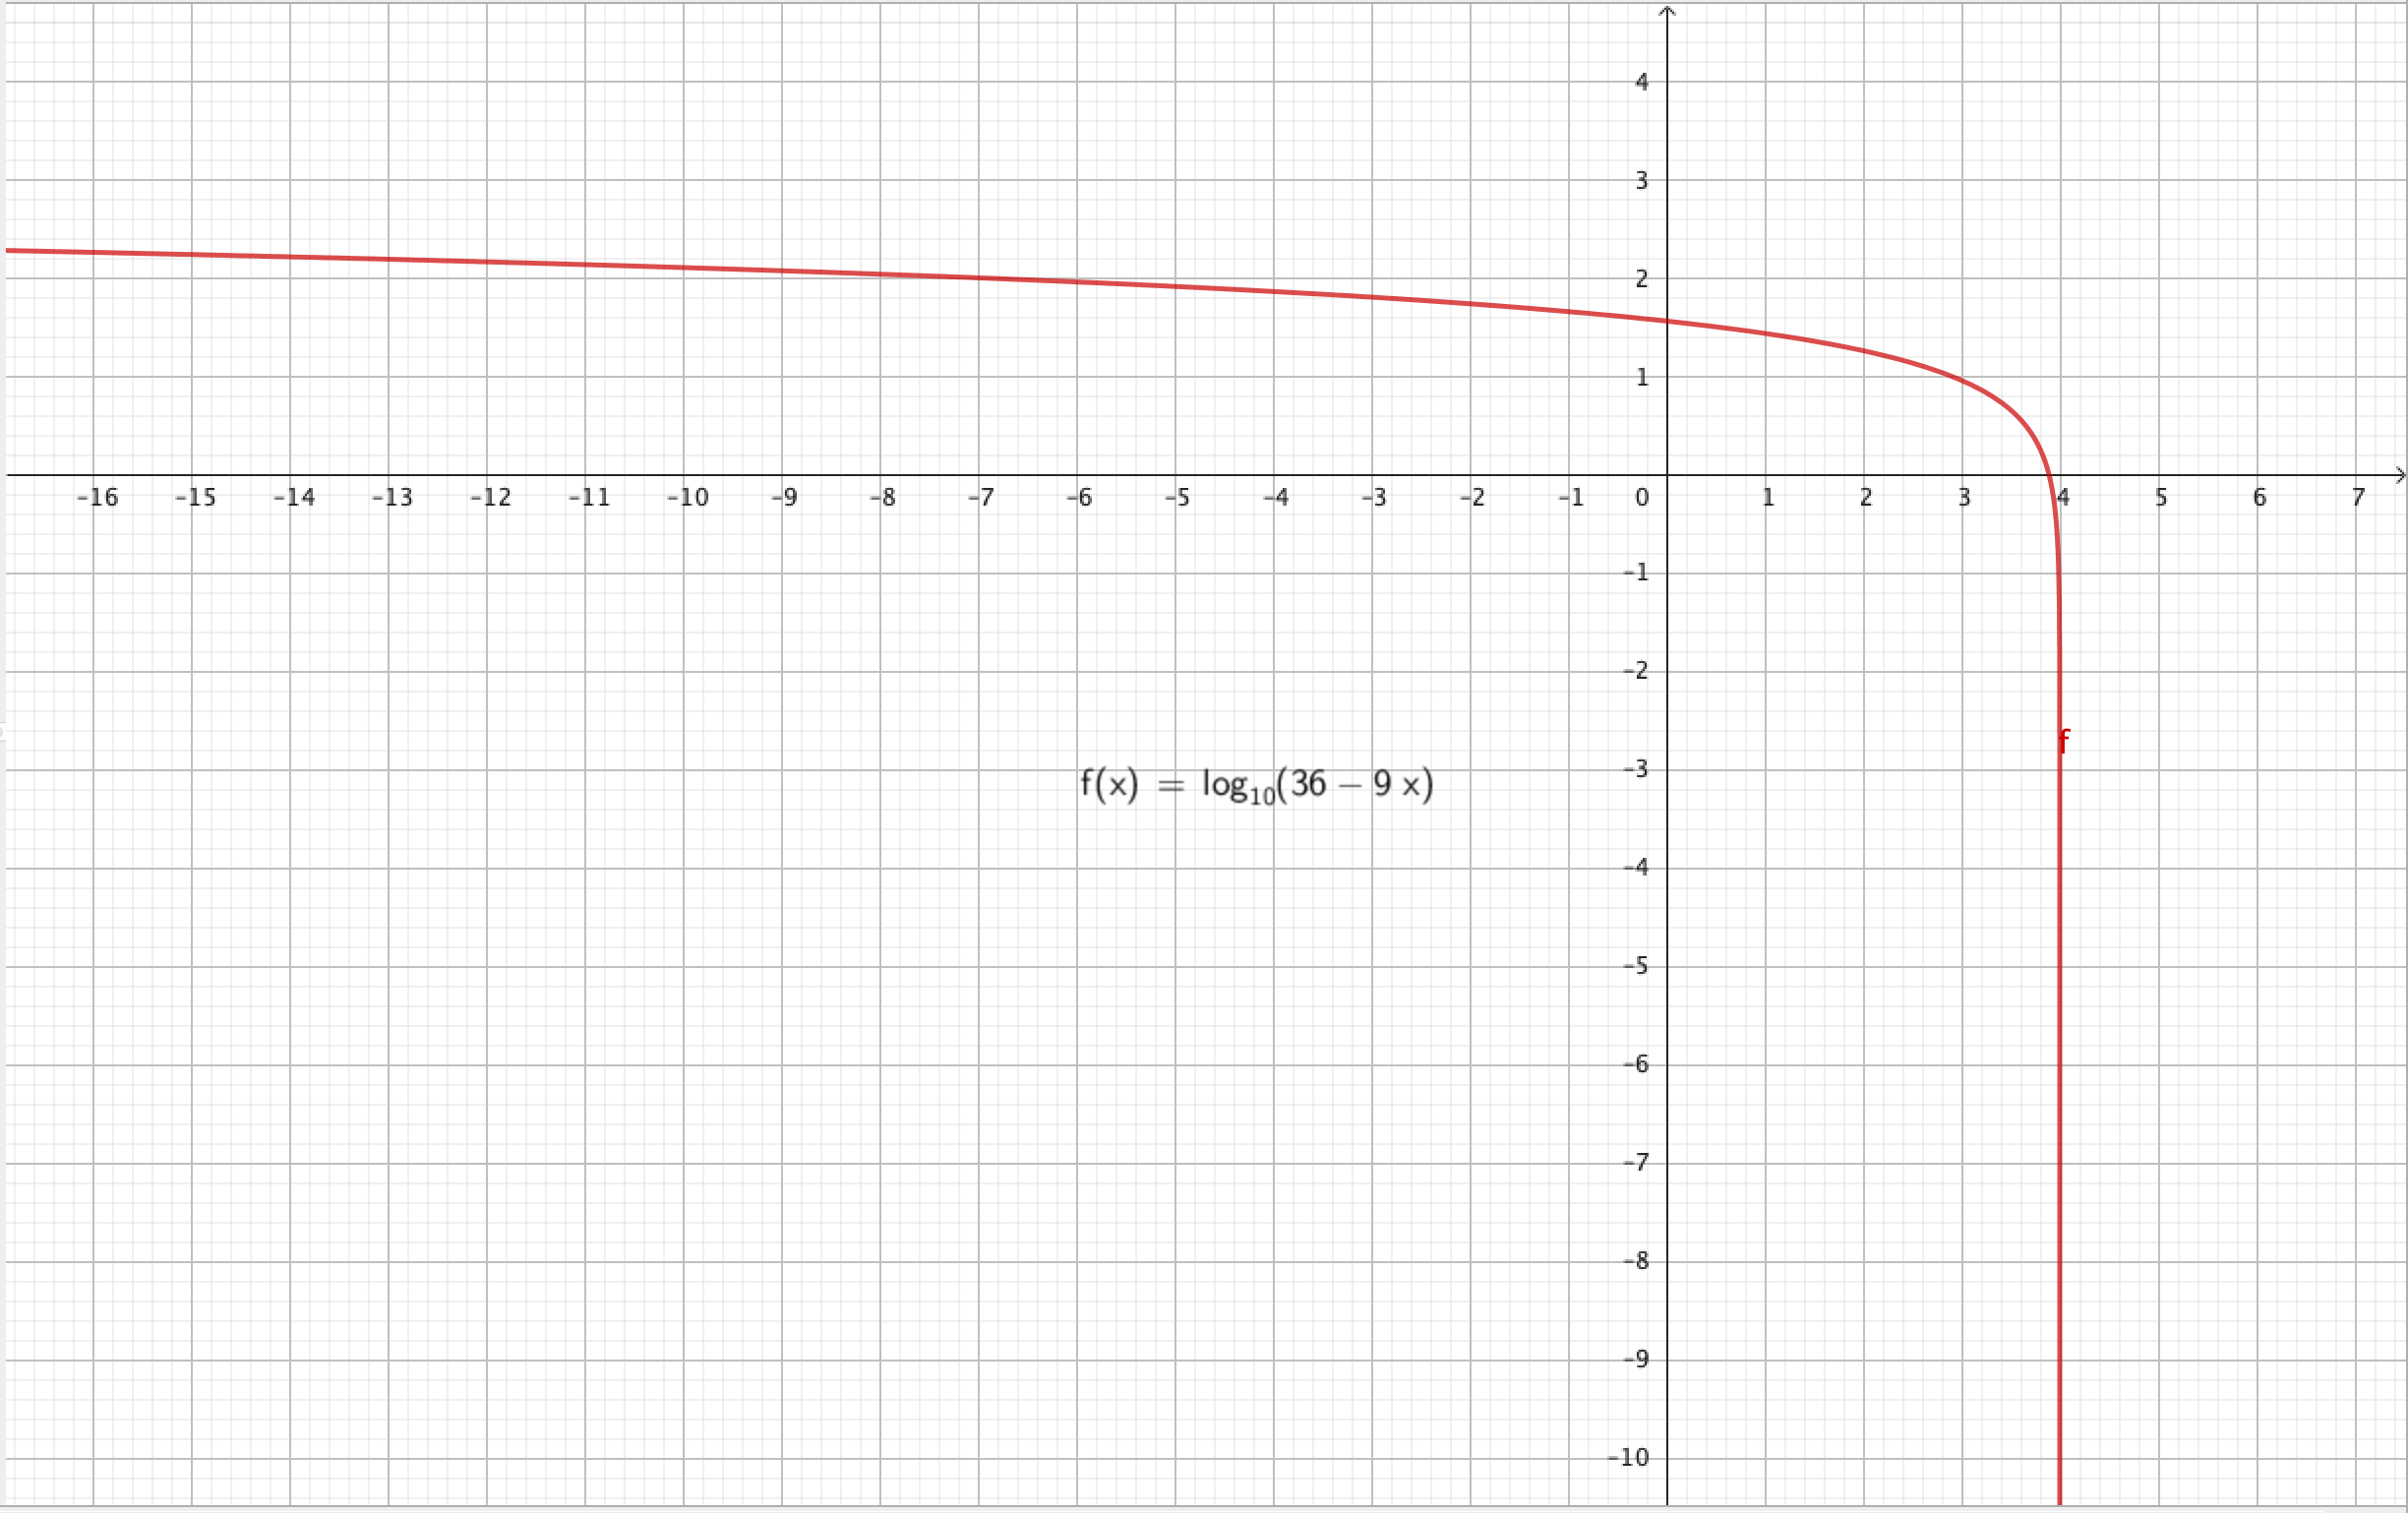
\includegraphics[width=\textwidth]{mat15graf.png}
\end{center}
\caption{Graf for $f$ tegnet i Geogebra}
\label{fig:f}
\end{figure}
\end{document} 
